% Georgetown Mathematics seminar, November 20, 2026.
% Compile from this directory:
%   pdflatex -interaction=nonstopmode ecatch-talk.tex
% Speaker notes are in \note{} on the teaching slides only.
% They are hidden in this PDF. To print them, add
% \setbeameroption{show notes} before \begin{document}.
%
% The manuscript \\includegraphics lines point these two files at each other's captions.
% The filenames match the pictures:
%   figure2_multimodal_fusion_architecture.pdf    = fusion heatmap
%   figure2_multimodal_temporal_integration.pdf   = temporal line chart
%
% 34 frames. Target: a 45-minute seminar, with time left for questions.

\documentclass[aspectratio=169,11pt]{beamer}

\usetheme{default}
\usecolortheme{default}
\setbeamertemplate{navigation symbols}{}
\setbeamersize{text margin left=7.5mm, text margin right=7.5mm}

\usepackage{amsmath,amssymb}
\usepackage{booktabs}
\usepackage{array}
\usepackage{tikz}
\usetikzlibrary{arrows.meta,positioning,calc}

\definecolor{gtown}{HTML}{041E42}
\definecolor{gtownmid}{HTML}{1F4B7A}
\definecolor{accent}{HTML}{8C6A1F}
\definecolor{soft}{HTML}{F3F6F8}
\definecolor{ink}{HTML}{14202B}
\definecolor{muted}{HTML}{5E6A75}
\definecolor{rule}{HTML}{C6A15B}

\setbeamercolor{normal text}{fg=ink,bg=white}
\setbeamercolor{structure}{fg=gtown}
\setbeamercolor{frametitle}{fg=white,bg=gtown}
\setbeamercolor{itemize item}{fg=gtown}
\setbeamercolor{itemize subitem}{fg=accent}
\setbeamercolor{enumerate item}{fg=gtown}
\setbeamerfont{frametitle}{series=\bfseries,size=\large}
\setbeamerfont{footline}{size=\scriptsize}

\setbeamertemplate{itemize item}{%
  \raise1.4pt\hbox{\color{gtown}\scriptsize\ensuremath{\blacksquare}}}
\setbeamertemplate{itemize subitem}{%
  \raise1.4pt\hbox{\color{accent}\scriptsize\ensuremath{\blacksquare}}}

\makeatletter
\setbeamertemplate{frametitle}{%
  \nointerlineskip%
  \vbox{%
    \hskip-\beamer@leftmargin%
    \begin{beamercolorbox}[%
        wd=\paperwidth,%
        leftskip=\beamer@leftmargin,%
        rightskip=\beamer@rightmargin]{frametitle}%
      \vskip0.62em%
      \usebeamerfont{frametitle}\insertframetitle\par%
      \ifx\insertframesubtitle\@empty\else
        {\usebeamerfont{framesubtitle}\insertframesubtitle\par}%
      \fi
      \vskip0.42em%
    \end{beamercolorbox}%
  }%
}
\setbeamertemplate{footline}{%
  \hbox{%
    \begin{beamercolorbox}[wd=.72\paperwidth,ht=2.35ex,dp=1.0ex,leftskip=7.5mm]{footline}%
      \color{muted}E-CaTCH \quad Georgetown Mathematics \quad November 20, 2026%
    \end{beamercolorbox}%
    \begin{beamercolorbox}[wd=.28\paperwidth,ht=2.35ex,dp=1.0ex,rightskip=7.5mm,right]{footline}%
      \color{muted}\insertframenumber\ /\ \inserttotalframenumber%
    \end{beamercolorbox}%
  }%
}
\makeatother

\newcommand{\R}{\mathbb{R}}
\newcommand{\MHAttn}{\mathrm{MHAttn}}

\graphicspath{{figures/}}

\title{E-CaTCH}
\author{Ahmad Mousavi}
\date{November 20, 2026}

\begin{document}

% ----- 1. Title -----
\setbeamercolor{background canvas}{bg=gtown}
\begin{frame}[plain]
  \color{white}
  \vspace*{0.22cm}
  \begin{center}
  {\fontsize{24}{28}\selectfont\bfseries E-CaTCH\par}
  \vspace{0.2cm}
  {\color{rule}\rule{3.4cm}{1.6pt}\par}
  \vspace{0.32cm}
  {\large
    Event-centric cross-modal attention\\[0.14em]
    with temporal consistency and class-imbalance handling\\[0.14em]
    for misinformation detection\par}
  \vspace{0.32cm}
  Ahmad Mousavi\\[0.12em]
  {\normalsize Department of Mathematics and Statistics, American University\par}
  \vspace{0.22cm}
  {\small
    Joint work with Yeganeh Abdollahinejad,
    Roberto Corizzo,\\
    Nathalie Japkowicz, and Zois Boukouvalas\par}
  \vspace{0.26cm}
  {\color{rule}
    Department of Mathematics, Georgetown University\\[0.1em]
    November 20, 2026\par}
  \vspace{0.18cm}
  {\footnotesize
    IEEE Transactions on Computational Social Systems, 2026\\
    \texttt{doi.org/10.1109/TCSS.2026.3693647}\par}
  \end{center}
\end{frame}
\setbeamercolor{background canvas}{bg=white}
\setbeamercolor{normal text}{fg=ink,bg=white}

% ----- 2. Problem -----
\begin{frame}{The story is larger than one post}
  \begin{itemize}
    \item A caption can read as ordinary until the picture is attached.
    \item A real photograph can still be paired with a false claim.
    \item Many posts carry one story, and the wording shifts over days.
    \item A score on a single post never sees that shift.
  \end{itemize}
  \vspace{0.8em}
  Misinformation here is multimodal, and it is a sequence.
\end{frame}

% ----- 3. Gaps -----
\begin{frame}{Three gaps in post-level detectors}
  \begin{enumerate}
    \item Joining a text vector to an image vector does not decide which modality to trust when they disagree.
    \item Models that score posts one by one miss how a narrative drifts inside an event.
    \item Real posts dominate. High accuracy can hide a miss on the rare class.
  \end{enumerate}
  \vspace{0.7em}
  The repair has three mathematical pieces: a gate, a short sequence of window vectors, and a weighted loss.
\end{frame}

% ----- 4. Claim -----
\begin{frame}{E-CaTCH reads an event, then a trend}
  Group related posts into a \emph{pseudo-event}.
  Fuse text and image with a coordinate-wise gate.
  Read the event as a short sequence of overlapping time windows.
  \vspace{0.7em}
  \begin{enumerate}
    \item Keep both cross-modal directions, then mix them with a gate.
    \item Track the change from one window to the next.
    \item Train with class weights, a temporal penalty, and $\ell_2$ regularization.
  \end{enumerate}
  \vspace{0.55em}
  {\small\color{muted}
    Plan for the hour: the vocabulary, the model, the three datasets, then the evidence.}
\end{frame}

% ----- 5. Post tuple -----
\begin{frame}{A post is four things}
  \begin{center}
    \begin{tikzpicture}[
      box/.style={draw=gtown, rounded corners=2pt, line width=0.7pt,
        fill=soft, minimum width=3.05cm, minimum height=1.35cm,
        align=center, font=\small}
    ]
      \node[box] (s) {text\\ $\mathbf{s}_i$};
      \node[box, right=0.38cm of s] (im) {image\\ $\mathbf{i}_i$};
      \node[box, right=0.38cm of im] (y) {label\\ $y_i\in\{0,1\}$};
      \node[box, right=0.38cm of y] (t) {time\\ $\tau_i$};
    \end{tikzpicture}
  \end{center}
  \vspace{0.35em}
  \[
    (\mathbf{s}_i,\ \mathbf{i}_i,\ y_i,\ \tau_i)
  \]
  \begin{itemize}
    \item $y_i$ is a post label: real or fake. The event label is not given.
    \item $\tau_i$ is the timestamp. Order is part of the data, not a feature we invent later.
  \end{itemize}
  \note{Walk the four coordinates slowly. Stress that the label is post-level and noisy, and that no event id sits in the tuple. We have to build events. Do not say ``BERT'' yet.}
\end{frame}

% ----- 6. Embedding -----
\begin{frame}{An embedding turns a post into a vector}
  \begin{center}
    \begin{tikzpicture}[
      box/.style={draw=gtown, rounded corners=2pt, line width=0.7pt,
        fill=soft, minimum width=3.1cm, minimum height=1.5cm, align=center}
    ]
      \node[box] (post) {text and image\\ of one post};
      \node[right=2.5cm of post, font=\Large] (vec) {$
        \begin{pmatrix} x_1 \\ x_2 \\ x_3 \\ \vdots \end{pmatrix}
        \in\R^{d}
      $};
      \draw[-{Stealth[length=2.6mm]}, line width=0.9pt, gtown]
        (post) -- (vec);
    \end{tikzpicture}
  \end{center}
  \vspace{0.2em}
  \begin{itemize}
    \item The coordinates are features, not words and not pixels.
    \item Posts the encoder treats as similar land near each other.
    \item Text and image each get a vector. A later linear map puts them in one shared $\R^{d}$.
  \end{itemize}
  \note{One picture, then stop. Nearby means similar to the encoder. Do not open a transformer, and do not explain training. The $x_i$ are placeholders.}
\end{frame}

% ----- 7. Encoders -----
\begin{frame}{Two frozen encoders, then a linear map}
  \begin{columns}[T,onlytextwidth]
    \begin{column}{0.49\textwidth}
      \textbf{BERT reads the text}\\[0.35em]
      A pretrained text encoder. We do not train it from scratch, and it is not ChatGPT.\\[0.45em]
      We keep one vector, the \texttt{[CLS]} embedding, in $\R^{768}$.
    \end{column}
    \begin{column}{0.49\textwidth}
      \textbf{ResNet-152 reads the image}\\[0.35em]
      A pretrained image network. We keep the vector before its classifier, in $\R^{2048}$.\\[0.45em]
      A missing image becomes the zero vector, so every post has the same shape.
    \end{column}
  \end{columns}
  \vspace{0.75em}
  A learned linear map sends both vectors into one dimension $d$:
  \[
    \mathcal{T}_i = W_{\mathrm{text}}\,\mathrm{BERT}_{\mathrm{CLS}}(\mathbf{s}_i)+b_{\mathrm{text}},
    \qquad
    \mathcal{I}_i = W_{\mathrm{img}}\,z_i+b_{\mathrm{img}}.
  \]
  {\small $W_{\mathrm{text}}\in\R^{d\times 768}$ and $W_{\mathrm{img}}\in\R^{d\times 2048}$. The encoders stay fixed; these two maps are trained.}
  \note{Say feature extractors, then $768$ and $2048$, then the shared $d$. If asked about a newer vision--language model: the encoders are held fixed so the hour stays on events, the gate, and the loss.}
\end{frame}

% ----- 8. Self-attention picture -----
\begin{frame}{Self-attention: each word looks at the others}
  \vspace{0.7em}
  \begin{center}
    \begin{tikzpicture}[word/.style={font=\Large, inner sep=2pt}]
      \node[word] (the) {The};
      \node[word, right=0.42cm of the] (photo) {photo};
      \node[word, right=0.42cm of photo] (shows) {shows};
      \node[word, right=0.42cm of shows] (a) {a};
      \node[word, right=0.32cm of a] (huge) {huge};
      \node[word, right=0.42cm of huge] (crowd) {crowd};
      \draw[-{Stealth[length=2.2mm]}, line width=0.8pt, accent]
        (huge.north) to[out=50,in=130,looseness=0.8] (crowd.north);
      \draw[-{Stealth[length=2.2mm]}, line width=0.8pt, gtownmid]
        (photo.north) to[out=62,in=118,looseness=1.05] (crowd.north);
    \end{tikzpicture}
  \end{center}
  \vspace{0.85em}
  \vspace{0.55em}
  \begin{itemize}
    \item ``Huge'' has to be licensed by ``crowd.'' ``Photo'' is pointing at the same noun.
    \item Each word builds a new vector as a weighted sum of the others.
    \item The weights are the attention. They depend on the words themselves.
  \end{itemize}
  \note{Read the sentence aloud. Ask which word ``huge'' depends on, then point at crowd. This is the only example. Do not define layers, residuals, or pretraining.}
\end{frame}

% ----- 9. Formula -----
\begin{frame}{One formula: scaled dot-product attention}
  \[
    \mathrm{Attention}(Q,K,V)
    = \mathrm{softmax}\!\left(\frac{QK^{\top}}{\sqrt{d_k}}\right) V
  \]
  \begin{itemize}
    \item $Q$, $K$, and $V$ are learned linear maps of the same sequence.
    \item Row $i$, column $j$ of $QK^{\top}$ is a score: how much token $i$ uses token $j$.
    \item Dividing by $\sqrt{d_k}$ keeps those scores from saturating the softmax.
    \item \textbf{Multi-head} means several of these maps in parallel. Their outputs are concatenated and mixed by one more matrix.
  \end{itemize}
  \note{Stay on this formula. If someone wants the matrix, point at $QK^{\top}$: rows are queries, columns are keys. The square root is a scale, nothing more. Do not derive backpropagation.}
\end{frame}

% ----- 10. Cross-attention -----
\begin{frame}{Cross-attention changes where the query comes from}
  \begin{columns}[T,onlytextwidth]
    \begin{column}{0.48\textwidth}
      \colorbox{soft}{\parbox[t]{\dimexpr\linewidth-2\fboxsep}{%
        \textbf{Text looks at the image}\\[0.35em]
        The query comes from the text.\\
        Keys and values come from the image.\\[0.45em]
        ``The streets are empty.''\\
        The picture is a packed square.\\[0.35em]
        Does the picture support the words?}}
    \end{column}
    \begin{column}{0.48\textwidth}
      \colorbox{soft}{\parbox[t]{\dimexpr\linewidth-2\fboxsep}{%
        \textbf{The image looks at the text}\\[0.35em]
        The query comes from the image.\\
        Keys and values come from the text.\\[0.45em]
        The same packed square.\\
        The same sentence about empty streets.\\[0.35em]
        Do the words describe this picture?}}
    \end{column}
  \end{columns}
  \vspace{0.7em}
  Both questions get an uncomfortable answer. We keep both answers.
  \note{Use the empty-street example once, slowly. The disagreement is the point. Say that nothing is discarded yet: the next slide is the decision. Do not write the cross-attention formula here.}
\end{frame}

% ----- 11. Why a gate -----
\begin{frame}{The gate chooses which direction to trust}
  Attention has already built two stories:
  what the text sees in the image, and what the image sees in the text.
  \vspace{0.7em}
  \begin{itemize}
    \item A weight near $1$ keeps the text-looks-at-the-image story.
    \item A weight near $0$ keeps the image-looks-at-the-text story.
    \item The weight is a \emph{vector}. Different coordinates may trust different modalities.
    \item The weight is chosen per post, from the two stories themselves.
  \end{itemize}
  \vspace{0.45em}
  Alignment finds the conflict. The gate decides the mix.
  \note{Empty streets versus a packed square. Near $1$ and near $0$ are enough. The formula comes after the pipeline. If asked: with one vector per side the softmax is trivial, and the gate does the mixing.}
\end{frame}

% ----- 12. Pipeline -----
\begin{frame}{Four blocks, then a decision}
  \vspace{-0.35em}
  \begin{center}
    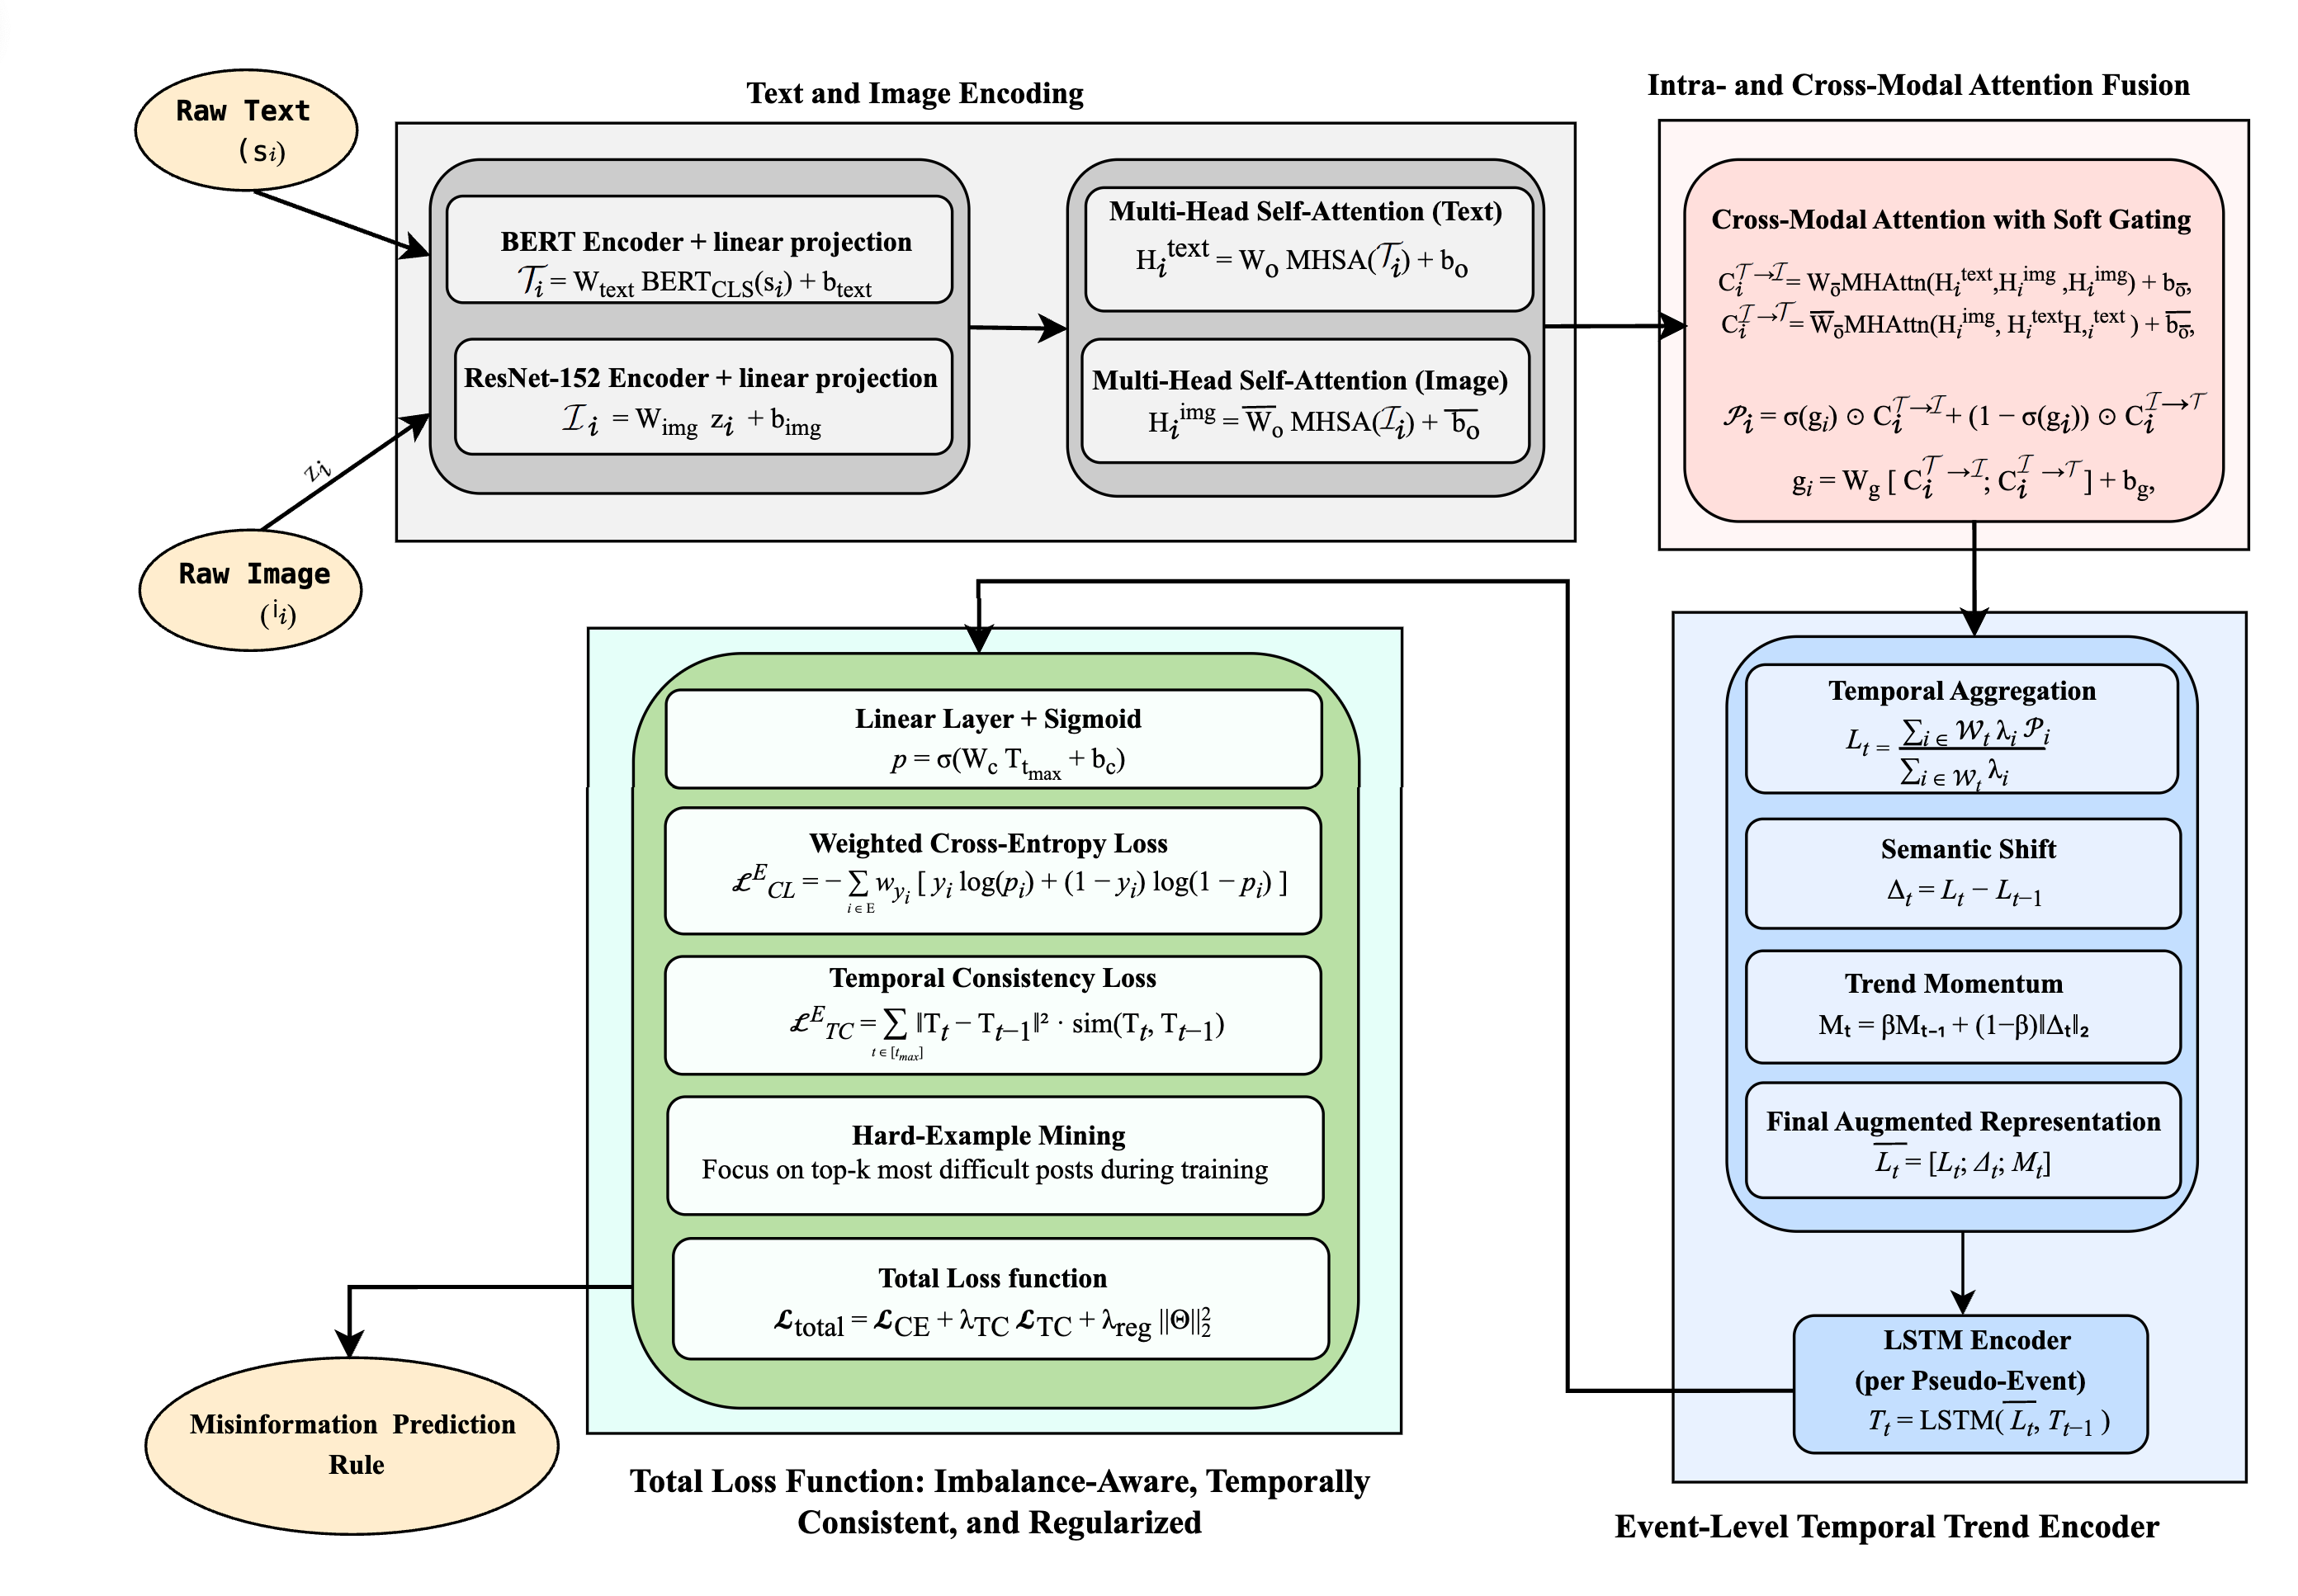
\includegraphics[width=\linewidth,height=0.74\textheight,keepaspectratio]{1212c.png}
  \end{center}
  \vspace{-0.15em}
  {\scriptsize\color{muted}
    Encoders, gated fusion, the temporal trend, and the loss.
    Figure from Mousavi et al., IEEE TCSS 2026.}
\end{frame}

% ----- 13. Clustering -----
\begin{frame}{Events are clusters we build, not labels we are given}
  \begin{itemize}
    \item Standardize sentence embeddings to mean zero and variance one.
    \item Agglomerative clustering, cosine distance, average linkage, \emph{inside each split}.
    \item Choose the number of clusters on validation, by event-level $F_1$.
    \item Images are used after the clusters exist. They do not define the clusters.
  \end{itemize}
  \vspace{0.35em}
  {\footnotesize
  \begin{center}
    \begin{tabular}{lccc}
      \toprule
      Clustering on Fakeddit & Silhouette $\uparrow$ & Davies--Bouldin $\downarrow$ & Intra-sim.\ $\uparrow$ \\
      \midrule
      Text only (BERT) & 0.37 & 1.05 & 0.64 \\
      Image only (ResNet) & 0.26 & 1.36 & 0.46 \\
      Text and image, concatenated & 0.32 & 1.18 & 0.57 \\
      \bottomrule
    \end{tabular}
  \end{center}
  }
  \vspace{0.25em}
  {\small Text wins every column. Images are often reused, missing, or weakly tied to the caption. The absolute scores are modest because the stream is noisy; the comparison is the evidence.}
\end{frame}

% ----- 14. Gate formula -----
\begin{frame}{The gate is a convex combination in each coordinate}
  Each modality vector is passed through the self-attention map, with that same vector as query, key, and value. Call the results $H_i^{\mathrm{text}}$ and $H_i^{\mathrm{img}}$.
  \vspace{0.35em}
  {\small
  \[
    C_i^{\mathcal{T}\to\mathcal{I}}
      = W\,\MHAttn(H_i^{\mathrm{text}},H_i^{\mathrm{img}},H_i^{\mathrm{img}})+b,
    \quad
    C_i^{\mathcal{I}\to\mathcal{T}}
      = \overline{W}\,\MHAttn(H_i^{\mathrm{img}},H_i^{\mathrm{text}},H_i^{\mathrm{text}})+\overline{b}.
  \]}
  \vspace{-0.35em}
  \[
    \mathcal{P}_i
    = \sigma(g_i)\odot C_i^{\mathcal{T}\to\mathcal{I}}
    + \bigl(1-\sigma(g_i)\bigr)\odot C_i^{\mathcal{I}\to\mathcal{T}}
  \]
  {\small
    $\sigma(g_i)\in(0,1)^{d}$, so coordinate $k$ of $\mathcal{P}_i$ is a convex combination of the two directions.
    The gate is $g_i = W_g \begin{bmatrix} C_i^{\mathcal{T}\to\mathcal{I}} \\ C_i^{\mathcal{I}\to\mathcal{T}} \end{bmatrix}+b_g$, with $W_g\in\R^{d\times 2d}$.
    With one vector on each side, the interesting mix is this gate.}
\end{frame}

% ----- 15. Windows -----
\begin{frame}{Inside an event, time is a row of overlapping windows}
  \begin{center}
    \begin{tikzpicture}[
      win/.style={draw=gtown, fill=soft, minimum width=3.5cm, minimum height=0.85cm, font=\small}
    ]
      \node[win] (w1) {window $t-1$};
      \node[win, right=1.35cm of w1] (w2) {window $t$};
      \draw[-{Stealth[length=2.2mm]}, gtownmid, line width=0.7pt] (w1) -- (w2);
      \node[below=0.45cm of w1, font=\scriptsize, align=center, text=muted]
        {posts ordered by $\tau$};
      \node[below=0.45cm of w2, font=\scriptsize, align=center, text=muted]
        {half of these posts\\ also sit in $t-1$};
    \end{tikzpicture}
  \end{center}
  \vspace{0.4em}
  \begin{itemize}
    \item Default overlap $\rho=0.5$: the stride is half a window, so neighbors share half their posts.
    \item The clock depends on the dataset. Fakeddit windows run about 3--5 days. The other two are set with their own data slides.
    \item Overlap keeps a gradual shift from falling into the crack between two windows.
  \end{itemize}
\end{frame}

% ----- 16. Decay, shift, momentum -----
\begin{frame}{Recent posts count more, and we record the jump}
  \begin{columns}[T,onlytextwidth]
    \begin{column}{0.49\textwidth}
      \centering
      \textbf{Inside window $t$}\\[0.55em]
      {\small $\displaystyle
        \lambda_i=\exp\!\bigl(-\alpha(\tau_{t,\max}-\tau_i)\bigr)
      $}\\[0.7em]
      {\small $\displaystyle
        L_t
        = \frac{\sum_{i\in\mathcal{W}_t}\lambda_i\,\mathcal{P}_i}
               {\sum_{i\in\mathcal{W}_t}\lambda_i}
      $}\\[0.65em]
      \parbox{0.46\textwidth}{\raggedright\small The newest post has weight $1$. Older posts in that window shrink. $\alpha>0$.}
    \end{column}
    \begin{column}{0.49\textwidth}
      \centering
      \textbf{From window $t-1$ to $t$}\\[0.55em]
      {\small $\displaystyle \Delta_t = L_t-L_{t-1}$}\\[0.85em]
      {\small $\displaystyle
        M_t = \beta M_{t-1}+(1-\beta)\,\|\Delta_t\|_2
      $}\\[0.7em]
      \parbox{0.46\textwidth}{\raggedright\small $\Delta_t$ is the change in the window summary. $M_t$ tracks the size of that change. $0<\beta<1$.}
    \end{column}
  \end{columns}
  \vspace{0.7em}
  The LSTM receives $\bar L_t=[L_t;\Delta_t;M_t]\in\R^{3d}$, with the scalar $M_t$ repeated across $d$ coordinates.
\end{frame}

% ----- 17. LSTM -----
\begin{frame}{An LSTM carries a state from window to window}
  \begin{center}
    \begin{tikzpicture}[
      win/.style={draw=gtown, fill=soft, rounded corners=2pt,
        minimum width=2.5cm, minimum height=0.9cm, font=\small},
      st/.style={draw=gtownmid, rounded corners=2pt,
        minimum width=2.1cm, minimum height=0.72cm, font=\scriptsize}
    ]
      \node[win] (w1) {window 1};
      \node[win, right=1.05cm of w1] (w2) {window 2};
      \node[win, right=1.05cm of w2] (w3) {window 3};
      \node[st, below=0.7cm of w1] (h1) {state $T_1$};
      \node[st, below=0.7cm of w2] (h2) {state $T_2$};
      \node[st, below=0.7cm of w3] (h3) {state $T_3$};
      \draw[-{Stealth}, gtown] (w1) -- (h1);
      \draw[-{Stealth}, gtown] (w2) -- (h2);
      \draw[-{Stealth}, gtown] (w3) -- (h3);
      \draw[-{Stealth}, accent, line width=0.7pt] (h1) -- (h2);
      \draw[-{Stealth}, accent, line width=0.7pt] (h2) -- (h3);
    \end{tikzpicture}
  \end{center}
  \vspace{0.25em}
  \begin{itemize}
    \item The event is a short sequence of windows. One new vector updates the state.
    \item The state and the cell start at $0$, and both are reset at every new event.
    \item We classify from $T_{T_E}$, the state after the last window.
  \end{itemize}
  \note{The picture is the whole explanation: input, state, pass it on, reset per event. If asked for backpropagation through time, defer. Sequences here are short, which is why a standard unidirectional LSTM is enough.}
\end{frame}

% ----- 18. Prediction and weights -----
\begin{frame}{One probability per event, with a class weight}
  \[
    p_E=\sigma(W_c T_{T_E}+b_c)
  \]
  The weight of class $c\in\{0,1\}$ is computed on events, not on posts:
  \[
    w_c=\frac{\bar n}{n_c+\varepsilon},
    \qquad
    \bar n=\frac{n_0+n_1}{2},
    \qquad \varepsilon>0.
  \]
  \[
    \mathcal{L}_{\mathrm{CE}}
    = -\sum_{E\in\mathcal{E}} w_{y_E}
      \bigl[y_E\log p_E+(1-y_E)\log(1-p_E)\bigr].
  \]
  The smaller class gets the larger weight. Training also emphasizes events whose loss is already large.
\end{frame}

% ----- 19. Event label -----
\begin{frame}{The event label comes from the last window}
  \[
    y_E
    = \mathbf{1}\!\left(
        \sum_{i\in\mathcal{W}_{T_E}} \lambda_i\, y_i
        \;\ge\;
        \frac12\sum_{i\in\mathcal{W}_{T_E}} \lambda_i
      \right)
  \]
  \begin{itemize}
    \item Only the most recent window votes, and recent posts inside it vote more.
    \item Early speculation in the same event does not get a vote.
    \item The displayed rule uses $\ge$. The paper also says a tie defaults to label $0$.
  \end{itemize}
  \vspace{0.4em}
  Event-level annotation is not in the data. This is the supervision the loss sees.
\end{frame}

% ----- 20. Total loss -----
\begin{frame}{The loss asks for fit, smoothness, and small weights}
  \[
    \mathcal{L}_{\mathrm{TC}}
    = \sum_{E\in\mathcal{E}}\sum_{t=2}^{T_E}
      \|T_t-T_{t-1}\|_2^2
      \cdot \mathrm{sim}(T_t,T_{t-1})
  \]
  $\mathrm{sim}$ is cosine similarity.
  The penalty is the squared step times the cosine of the angle between neighboring states.
  \vspace{0.45em}
  \[
    \mathcal{L}_{\mathrm{total}}
    = \mathcal{L}_{\mathrm{CE}}
    + \lambda_{\mathrm{TC}}\,\mathcal{L}_{\mathrm{TC}}
    + \lambda_{\mathrm{reg}}\,\|\Theta\|_2^2
  \]
  $\Theta$ is the set of trainable parameters. Each term is computed at event level.
\end{frame}

% ----- 21. Fakeddit -----
\begin{frame}{Fakeddit: a large Reddit stream, with no event labels}
  \begin{itemize}
    \item About $1.2$ million Reddit posts, text and image, real or fake.
    \item Topics are mixed: politics, entertainment, and much else.
    \item Events are not annotated. Pseudo-events come from the clustering step.
    \item Inside a cluster, posts are ordered by time and cut into windows of about 3--5 days.
    \item Overlap $\rho=0.5$.
    \item Misinformation is the minority class, as it is on the other two sets.
  \end{itemize}
\end{frame}

% ----- 22. IND -----
\begin{frame}{IND: fact-checked images from Indian elections}
  Fact-Checked Images Shared During Elections.
  \vspace{0.55em}
  \begin{itemize}
    \item Campaign material from 2013--2021. Each item is a claim plus an image, real or fake.
    \item Moderately sized, and strongly imbalanced: misinformation is about $20\%$ of the samples.
    \item Daily windows, overlap $\rho=0.5$, in step with a political news cycle.
    \item Explicit event labels are not provided, so the same pseudo-event construction applies.
  \end{itemize}
\end{frame}

% ----- 23. COVID -----
\begin{frame}{MediaEval 2020: COVID-19 tweets}
  The MISINFOGRAPH task from MediaEval 2020.
  \vspace{0.55em}
  \begin{itemize}
    \item Pandemic-related tweets, labeled misleading or accurate.
    \item Mostly text, with some images.
    \item Weekly windows, overlap $\rho=0.5$.
    \item Health narratives move more slowly than election news, so the window is longer.
    \item Misinformation is again the minority class.
  \end{itemize}
  \vspace{0.4em}
  Three platforms, three clocks, one overlap rule.
\end{frame}

% ----- 24. Protocol -----
\begin{frame}{One protocol on all three datasets}
  \begin{itemize}
    \item Split $80/10/10$ into train, validation, and test.
    \item Clustering and windowing are fit \emph{inside} each split, so posts from one story do not leak across the cut.
    \item Every number below is a mean $\pm$ standard deviation over $5$ seeds.
    \item Hyperparameters are chosen on validation only. The test set is scored once.
    \item When two model variants are compared, they share encoders, windows, optimizer, and class weights. Only the piece under study changes.
    \item Misinformation is the minority class on all three. That is the realistic setting, and the class weight is there because of it.
  \end{itemize}
\end{frame}

% ----- 25. Main results -----
\begin{frame}{The same model on three datasets}
  {\small
  \begin{center}
    \renewcommand{\arraystretch}{1.18}
    \begin{tabular}{lccccc}
      \toprule
      Dataset & Accuracy (\%) & Precision & Recall & $F_1$ & AUC \\
      \midrule
      Fakeddit & $95.5\pm 0.30$ & $0.957\pm 0.006$ & $0.953\pm 0.009$ & $0.955\pm 0.008$ & $0.975\pm 0.004$ \\
      IND & $89.8\pm 0.36$ & $0.903\pm 0.009$ & $0.890\pm 0.011$ & $0.896\pm 0.010$ & $0.925\pm 0.005$ \\
      COVID-19 & $89.5\pm 0.38$ & $0.899\pm 0.007$ & $0.885\pm 0.010$ & $0.891\pm 0.009$ & $0.938\pm 0.005$ \\
      \bottomrule
    \end{tabular}
  \end{center}
  }
  \vspace{0.7em}
  Fakeddit is the largest and most mixed, and it is where the model is strongest.
  IND and the COVID-19 set are harder, and both are minority-class problems.
  The paper reports a $1.57$ percentage-point accuracy gain on Fakeddit over prior strong baselines.
\end{frame}

% ----- 26. Baselines -----
\begin{frame}{On Fakeddit, against published multimodal models}
  {\footnotesize
  \begin{center}
    \renewcommand{\arraystretch}{1.12}
    \begin{tabular}{lcccc}
      \toprule
      Model & Accuracy (\%) & Precision & Recall & $F_1$ \\
      \midrule
      EANN   & 87.5 & 0.9043 & 0.8811 & 0.8926 \\
      MVAE   & 88.8 & 0.9011 & 0.9139 & 0.9074 \\
      ELD-FN & 88.8 & 0.9354 & 0.9029 & 0.9189 \\
      MMBT   & 91.1 & 0.9274 & 0.9251 & 0.9263 \\
      MTTV   & 91.9 & 0.9348 & 0.9303 & 0.9325 \\
      BMR    & 91.7 & 0.9434 & 0.9288 & 0.9361 \\
      GAMED  & 93.9 & 0.9355 & 0.9371 & 0.9363 \\
      \textbf{E-CaTCH} & \textbf{95.5} & \textbf{0.9570} & \textbf{0.9530} & \textbf{0.9550} \\
      \bottomrule
    \end{tabular}
  \end{center}
  }
  \vspace{0.35em}
  {\scriptsize\color{muted}
    EANN adversarial; MVAE generative; ELD-FN event-level fusion; MMBT early fusion;
    MTTV temporal transformer; BMR multi-view; GAMED multi-expert.
    Same table as the paper. Best entry in each column is ours.}
\end{frame}

% ----- 27. Fusion -----
\begin{frame}{Adaptive fusion is best on every dataset}
  \vspace{-0.45em}
  \begin{center}
    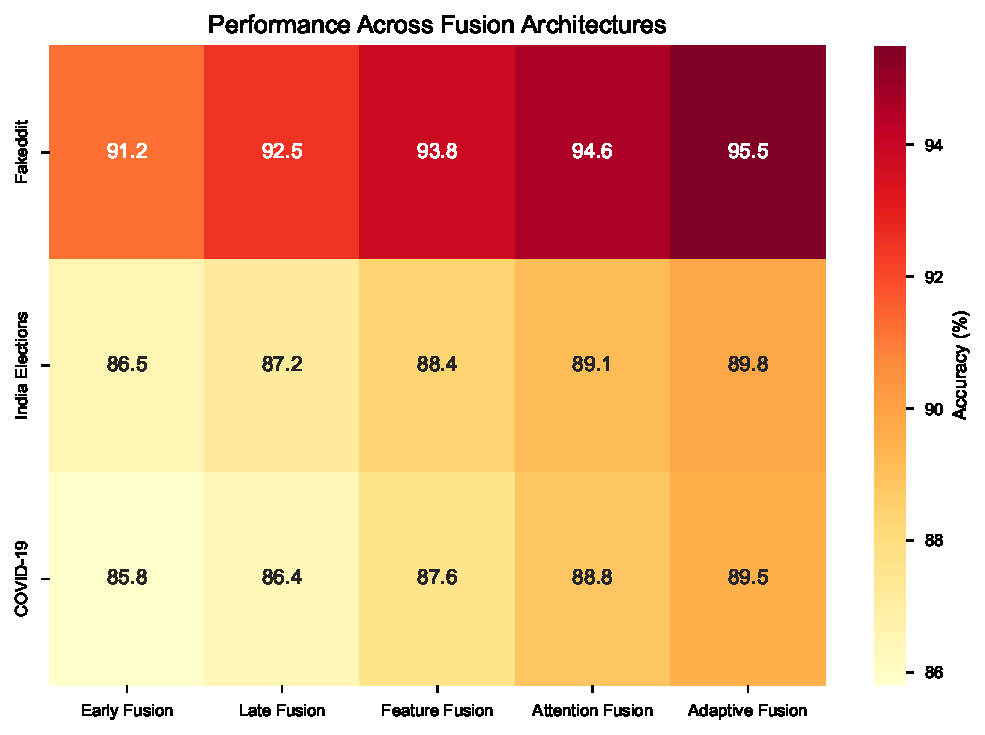
\includegraphics[width=0.72\linewidth,height=0.56\textheight,keepaspectratio]{figure2_multimodal_fusion_architecture.pdf}
  \end{center}
  \vspace{0.15em}
  {\scriptsize\color{muted}
    Only the fusion block changes.
    Early fusion to adaptive fusion, as printed: $91.2\to 95.5$, $86.5\to 89.8$, $85.8\to 89.5$.}
\end{frame}

% ----- 28. Temporal -----
\begin{frame}{Time lifts each modality; both together sit at the top}
  \vspace{-0.4em}
  \begin{center}
    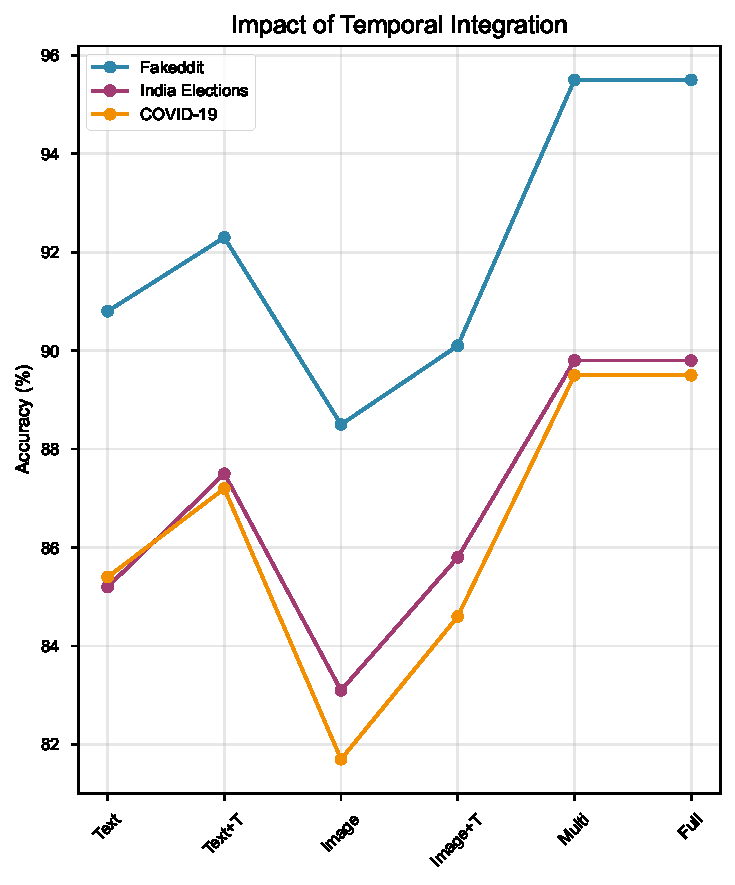
\includegraphics[width=0.72\linewidth,height=0.60\textheight,keepaspectratio]{figure2_multimodal_temporal_integration.pdf}
  \end{center}
  \vspace{-0.2em}
  {\scriptsize\color{muted}
    Text, text plus time, image, image plus time, multimodal, full model.
    On each curve the image-only point is lowest, time lifts text and lifts image, and the multimodal and full models sit together above either modality.}
\end{frame}

% ----- 29. Ablation -----
\begin{frame}{Removing a module lowers accuracy}
  \vspace{-0.45em}
  \begin{center}
    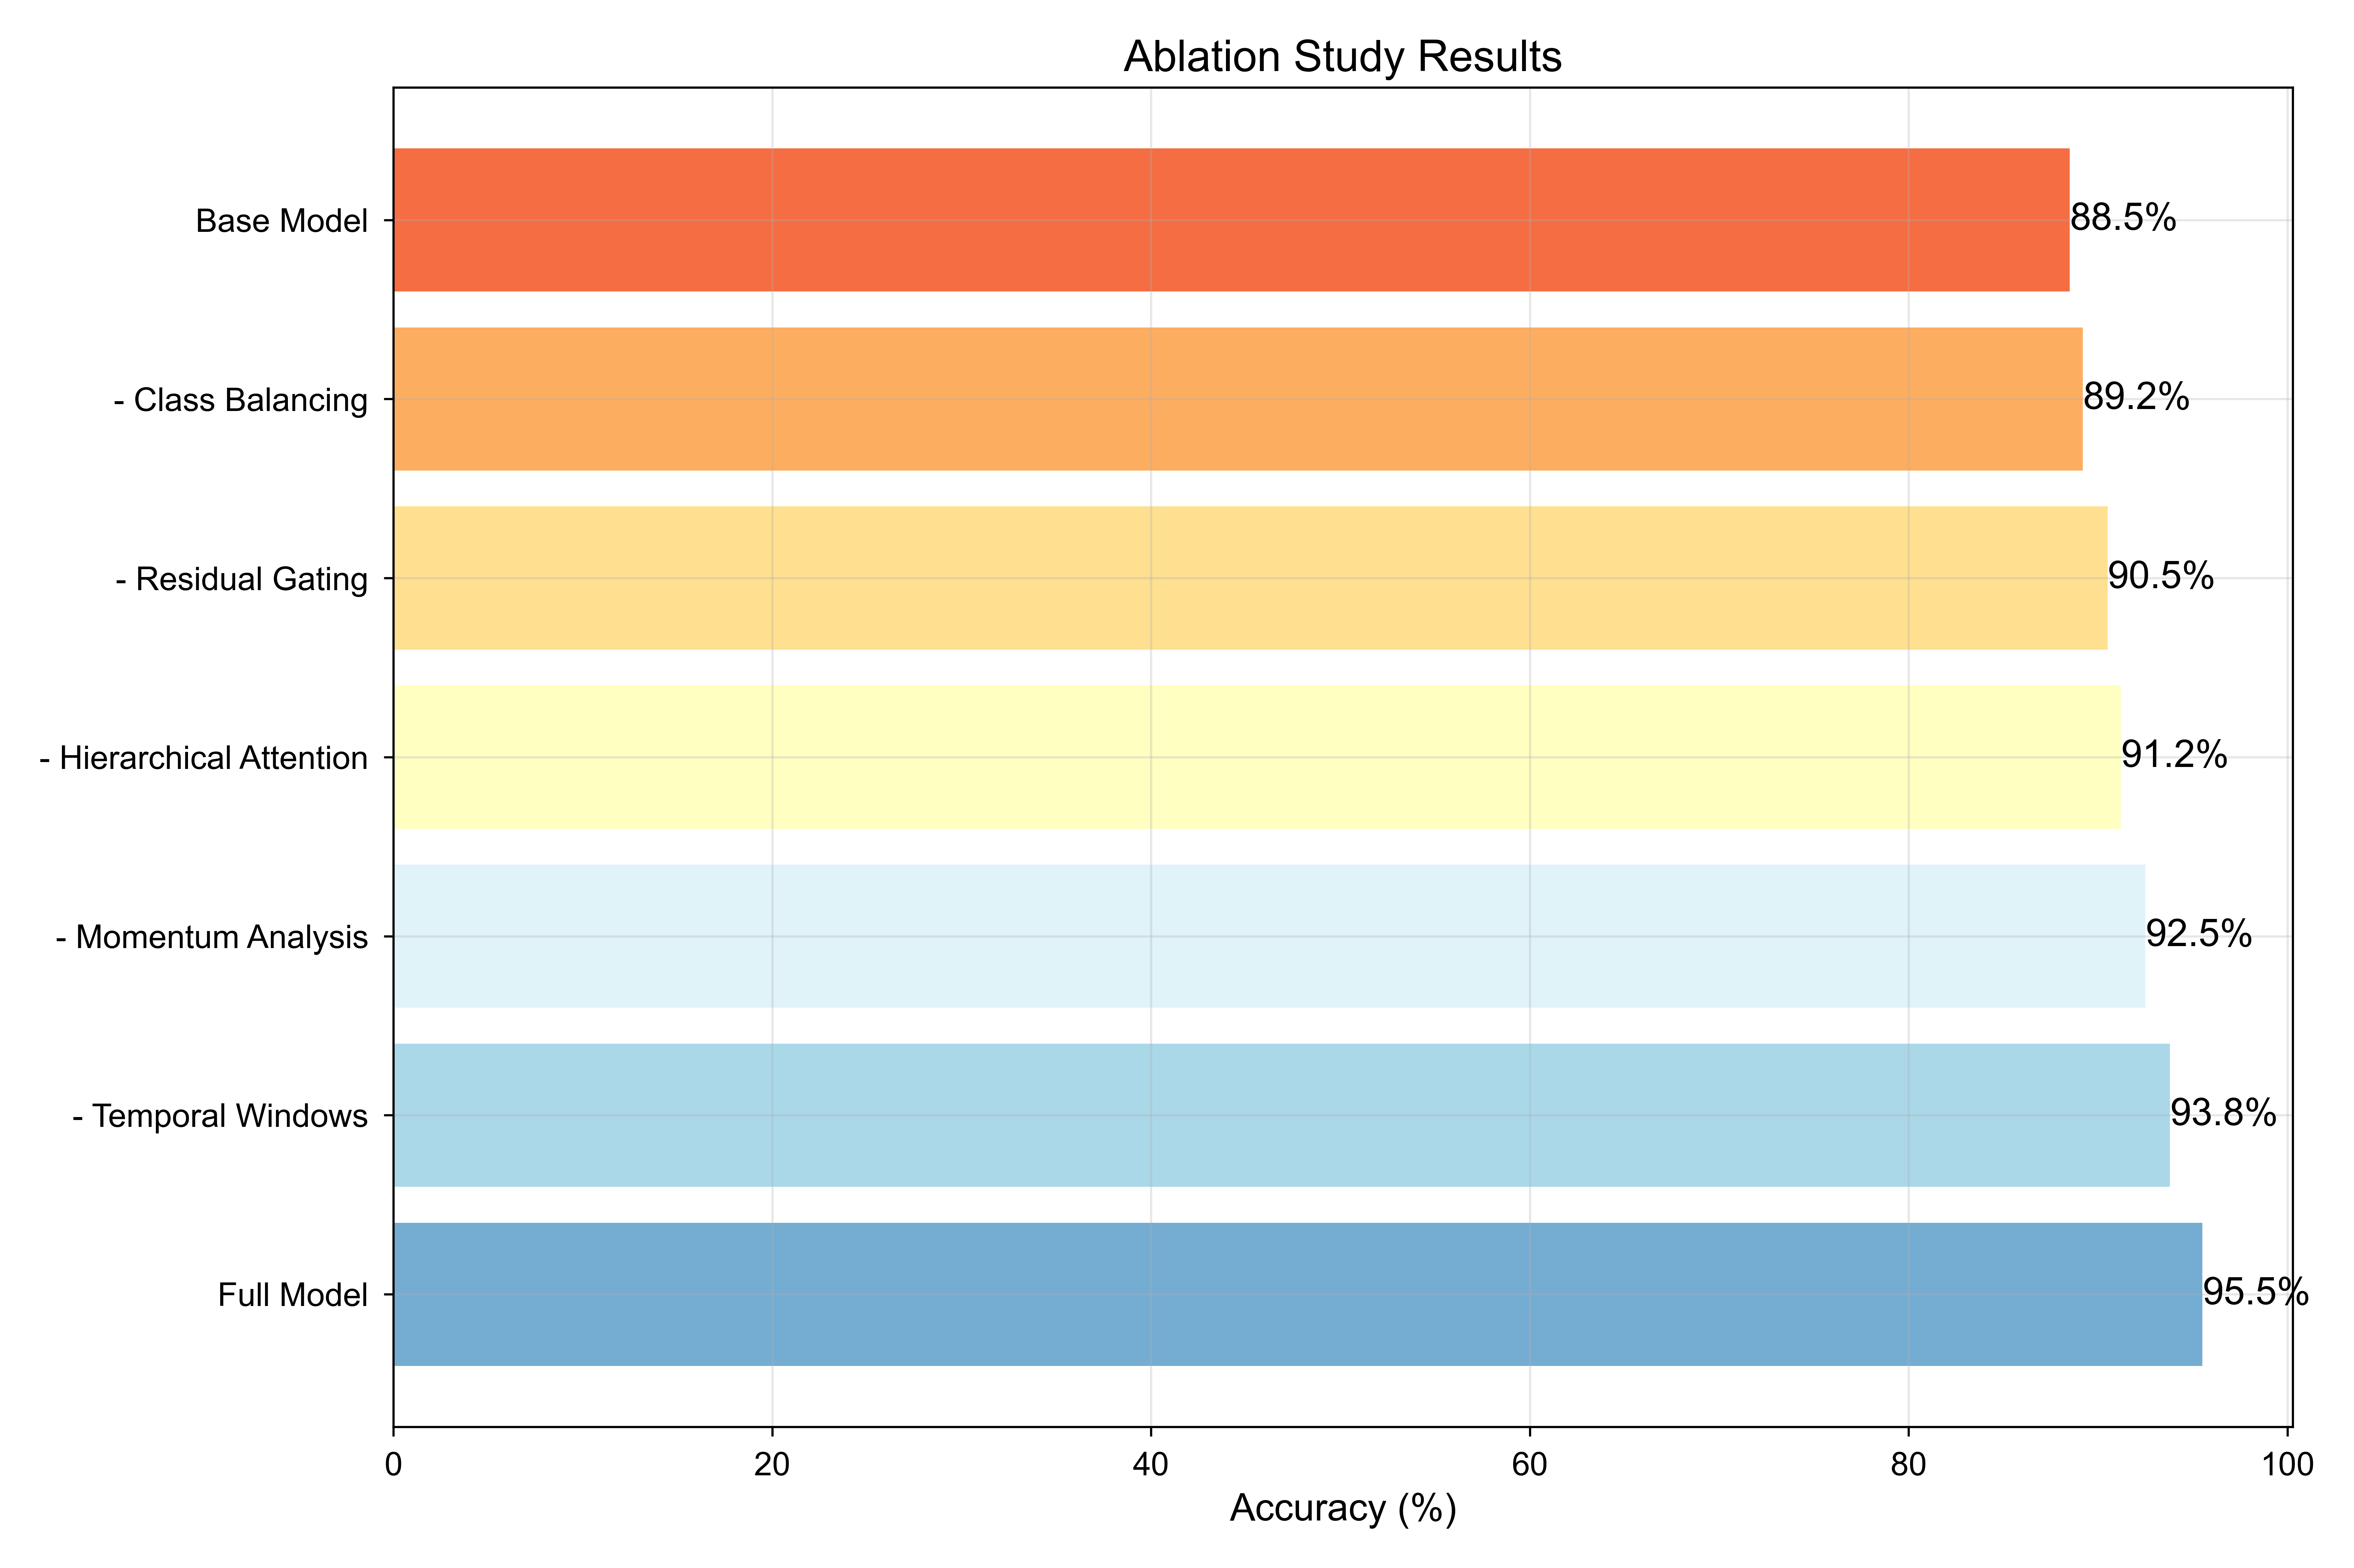
\includegraphics[width=0.88\linewidth,height=0.58\textheight,keepaspectratio]{ablation_study.png}
  \end{center}
  \vspace{-0.2em}
  {\scriptsize\color{muted}
    Each intermediate bar disables one module. The figure prints a base model at $88.5\%$ and the full model at $95.5\%$.
    Class balancing removed: $89.2\%$. Temporal windows removed: $93.8\%$.
    Class balancing is the adaptive weight; residual gating is the soft gate.}
\end{frame}

% ----- 30. Rho -----
\begin{frame}{Overlap near one half is a stable default}
  \vspace{-0.4em}
  \begin{center}
    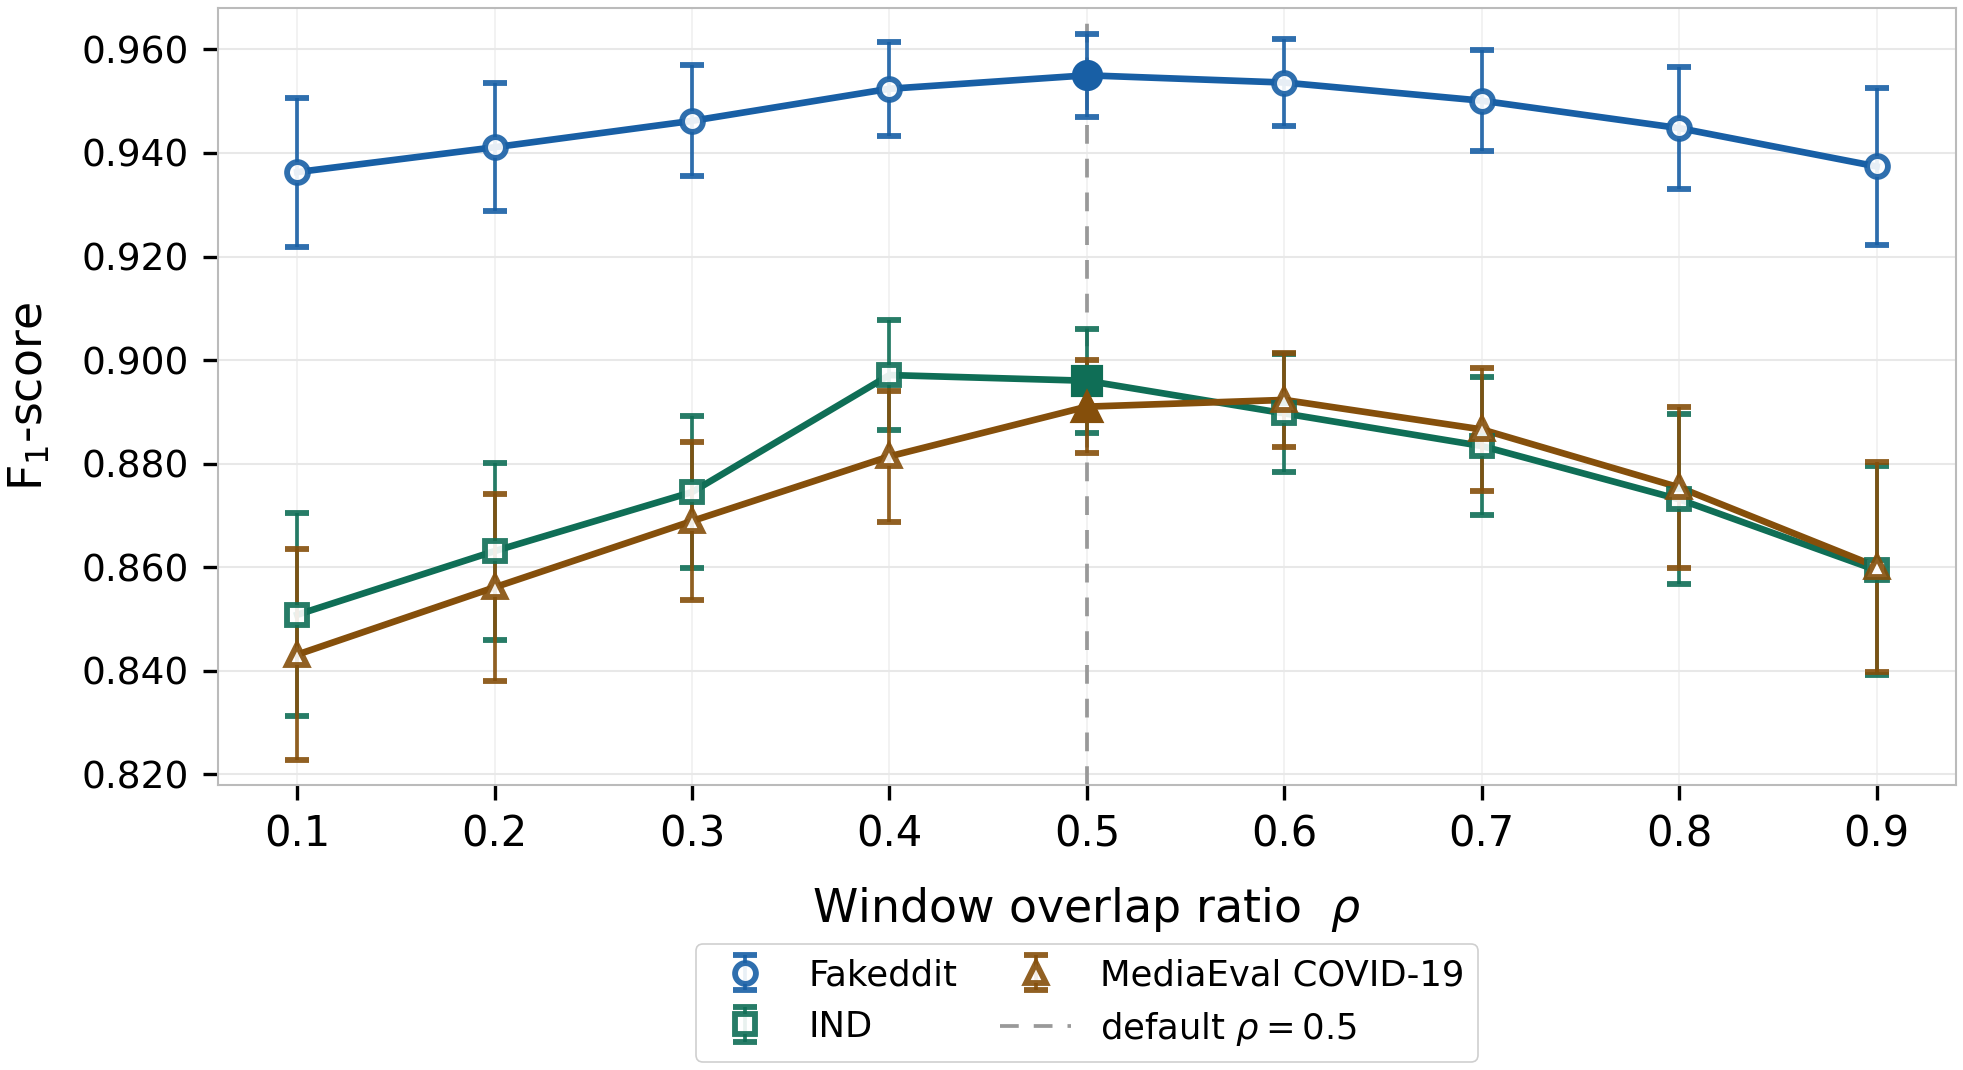
\includegraphics[width=0.80\linewidth,height=0.56\textheight,keepaspectratio]{rho_f1_exact.png}
  \end{center}
  \vspace{-0.15em}
  {\scriptsize\color{muted}
    $F_1$ stays stable for $\rho$ from $0.4$ to $0.6$.
    Fakeddit peaks at $0.5$. IND is slightly higher at $0.4$, and COVID-19 at $0.6$; both gaps from $0.5$ sit inside the run-to-run deviation.
    The extremes $0.1$ and $0.9$ are weaker. The main experiments use $\rho=0.5$.}
\end{frame}

% ----- 31. Transfer -----
\begin{frame}{Train on one platform, test on another}
  No fine-tuning. Hyperparameters stay at the source dataset.
  \vspace{0.6em}
  \begin{center}
    \renewcommand{\arraystretch}{1.2}
    \begin{tabular}{lc}
      \toprule
      Train $\to$ test & Accuracy (\%) \\
      \midrule
      Fakeddit $\to$ IND & $88.2\pm 0.40$ \\
      Fakeddit $\to$ COVID-19 & $87.8\pm 0.42$ \\
      IND $\to$ Fakeddit & $89.5\pm 0.38$ \\
      COVID-19 $\to$ Fakeddit & $89.1\pm 0.39$ \\
      \bottomrule
    \end{tabular}
  \end{center}
  \vspace{0.7em}
  A model trained on Reddit still lands near $88\%$ on election images and on COVID-19 tweets.
\end{frame}

% ----- 32. Limits -----
\begin{frame}{Where the method is thin}
  \begin{itemize}
    \item Clustering uses text only. Memes and posts with almost no caption can be split across events.
    \item A point-in-time event gives the temporal branch little signal. The model then falls back to a stable event vector.
    \item Audio, video, external knowledge, social graphs, and a measured inference cost are open.
  \end{itemize}
  \vspace{0.6em}
  The gate is a per-post reading of which direction was trusted. Using that reading as a display for fact-checkers is future work, not a result in this paper.
\end{frame}

% ----- 33. Takeaways -----
\begin{frame}{Three things to keep}
  \begin{enumerate}
    \item The unit is the event we build from text and time, not the isolated post.
    \item Keep both cross-modal directions. Mix them with a convex combination in each coordinate.
    \item A short sequence of windows, with decay, shift, and momentum, is enough time structure when the loss respects class imbalance.
  \end{enumerate}
  \vspace{0.8em}
  On that design: $95.5\%$ accuracy on Fakeddit, $89.8\%$ on IND, and $89.5\%$ on the COVID-19 set.
\end{frame}

% ----- 34. Questions -----
\begin{frame}{Questions}
  \vspace{0.4em}
  {\Large I would like to leave the rest of the hour for questions.}
  \vspace{1.1em}
  \begin{itemize}
    \item The gate, the event label, and the text-only clustering are the pieces I am happiest to unpack.
  \end{itemize}
  \vspace{1.2em}
  {\small
    Mousavi, Abdollahinejad, Corizzo, Japkowicz, and Boukouvalas.\\
    IEEE Transactions on Computational Social Systems, 2026.\\
    \texttt{doi.org/10.1109/TCSS.2026.3693647}\\[0.35em]
    Code: \texttt{github.com/Yegi03/E-CaTCH}}
\end{frame}

\end{document}
